% !TeX spellcheck = <none>
%\chapter{Radar frame processing}
%\label{chap:radar_detection}

	\section{Radar search and detection}
	\label{sec:radar_search_detection}
		Detection is commonly defined as the process of analysing the radar data and determining whether it consists of noise only, or noise plus echoes coming from a target of interest \cite{Richards_Scheer_Holm_2010}. 
		The first hypothesis is denoted as the null hypothesis $H_0$ and the second as the non-null hypothesis $H_1$.
		Detection is achieved by setting a threshold for the region of interest, based on the level of interference, and deciding whether any part of that region is "bright" enough compared to the background.
		
		%TODO generate image showing fixed vs adaptive threshold
		
		Radar users are typically concerned with determining (or defining) the probability of detecting a target $P_\text{D}$ and the probability of false alarm $P_\text{{FA}}$.  By utilizing the knowledge of the desired $P_\text{{FA}}$, noise statistics, and detector design, it is possible to decide the appropriate threshold level to be used at the detector's output.
		
		% TODO asses feasibility of confirmation system (does not work for clutter)
		
		
		
		% TODO consider putting something about clutter statistics
		
		In this work different approaches were be considered and their respective advantages and drawbacks analysed. 



		\subsection{Constant False Alarm Rate}
	
				Standard radar detection assumes the level of noise and interference to be known and constant. In this conditions it is possible to precisely determine the correct threshold for achieving the desired $	p_\text{FA}$. In real scenarios interference levels may be highly variable throughout an acquisition, making the use of a dynamic threshold necessary. Constant false alarm rate (CFAR) is an adapting threshold technique aiming at providing predictable behaviour of detection and false alarm rates in real scenarios.
				
				%TODO generate image showing fixed vs adaptive threshold
				
				In OFDM radar, a \textit{false alarm} occurs when the target detector determines the presence of a target at a range and relative speed that does not contribute to the received matrix $\bm{F}_{Rx}$ \cite{Braun2014OFDMRA}. 
				Consequently, the probability of false alarm is the probability of observing a positive detection when the received frame consists only of noise $(\bm{F}_{Rx} = \bm{Z})$. 
				This definition considers processing on a per-frame basis and can also be applied to the multi-frame processing strategies presented in chapter \ref{chap:TDD pattern of the OFDM frame}. 
				
				The presence of clutter is not yet taken into account as the threshold is estimated by determining an estimator for the noise power of the processed data. 
				Furthermore, clutter can be defined as reflections generated by objects in the environment, that are not of interest for the sensing task. 
				This means that detections due to objects considered as clutter are expected and can be mitigated by various clutter removal techniques.
				
				In order to discriminate noise from signal power, the periodogram is subjected to an hypothesis test with an appropriate threshold
				
				\begin{align*}
					\text{Per}_{\bm{F}}(n,m) \quad\mathop{\gtrless}_{H_1}^{H_0}  \quad \eta,
				\end{align*}
				
				where $H_0$ is the null hypothesis, target not present, and $H_1$ is the hypothesis where the reflection from a target contributes to the received power in the bin under test.\\
				The probability that any bin of the periodogram exceeds the threshold when only noise power $Z$ is present is
				
				\begin{align*}
					p_{\text{FA},bin} = \text{Per}(Z > \eta) = \int_\eta^{\infty} f_z(z|H_0)dz = 1 - F_z(\eta | H_0) = e^{-\dfrac{\eta}{\sigma_n^2}},
				\end{align*}
				 
				where $f_z(z|H_0)$ and $F_z(\eta | H_0)$ are the PDF and CDF of the random variable $Z$. 
				The observed noise contribution is given by the magnitude squared of the AWGN with power $\sigma_n^2$.
				 
				The threshold for a given false alarm rate per bin is obtained as
				
				\begin{align*}
					\eta = -\sigma_n^2 \ln(p_{\text{FA},bin}) .
				\end{align*} 
				
				Optimality for this detection method and a more thorough theoretical analysis can be found in chapter 15 of \cite{Richards_Scheer_Holm_2010}.
				For the full (non zero padded) periodogram the false alarm probability is
				
				\begin{align*}
					p_\text{FA} = 1 - (1 - p_{\text{FA},bin})^{NM}.
				\end{align*}
				
				Solving this for $p_{\text{FA},bin}$ we obtain the value of the threshold as 
				
				\begin{align*}
					\eta = \sigma_N^2 \ln{(1 - (1 - p_{\text{FA},bin})^{\frac{1}{NM}})}.
				\end{align*}
				
				Zero padding the periodogram does not add information useful for the target estimation problem, but it only reduces quantization noise. The contribution of a single bin is spread out between multiple contiguous bins when zero padding.

				\subsubsection{Estimation of noise power}
	
					Noise power is estimated from the periodogram averaging over bins where the target is not expected.
					
					From Assumption 3 from section \ref{sub:assumptions_ofdm_radar}, the maximum target delay and consequently the maximum range bin in which we can observe a target depend on the guard interval defined by the \gls{cp}, and are given by
					\begin{align*}
						\tau_{\text{max}} =& \frac{N_{\text{max}}}{N_{\text{Per}}}\cdot T = T_\text{CP} ,\\
						N_{\text{max}} =& \frac{T_\text{CP}}{T}\cdot N_{\text{Per}}.
					\end{align*} 
					
					The maximum likelihood estimate for the noise power is found by averaging over one or more rows beyond $N_{\text{max}}$
			
					\begin{align}
					\label{align: threshold_noise_power}
						\hat{\sigma_N}^2 = \frac{1}{M_{\text{Per}}K} \sum_{k=1}^K \sum_{m=1}^{M_{\text{Per}}} \text{Per}_{\bm{F}}(N_{\text{max}}+k, m).
					\end{align}
			
			Standard CFAR is an established method, howeverit was observed that estimating a fixed threshold across the periodogram based only on the level of the noise floor leads numerous above-threshold cells due to the sidelobes of the target returns, as shown in Figure \ref{fig:RadThesh_CFAR_abv_thresh_doubl}.
			
				\begin{figure}[H]
				\centering
				
				\subfloat[Above-threshold bins, threshold estimated using CFAR.\label{fig:RadThesh_CFAR_abv_thresh}]{%
					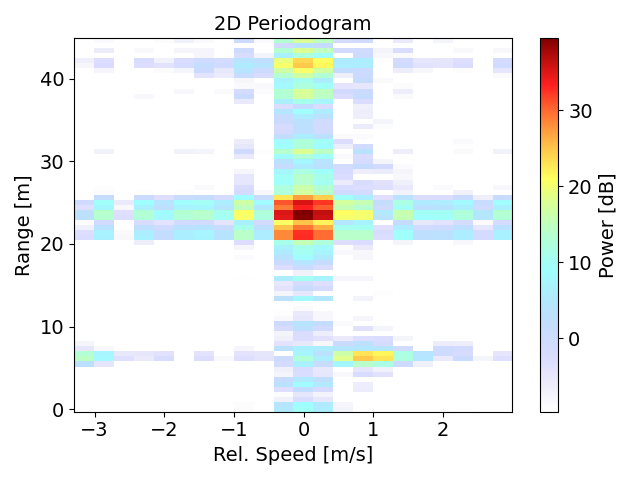
\includegraphics[scale=0.45]{Images/radar_detect_threshold/cfar_abv_thresh.png}%
				}\hfill
				\subfloat[Reference periodogram. \label{fig:RadThesh_CFAR_abv_thresh_PER}]{%
					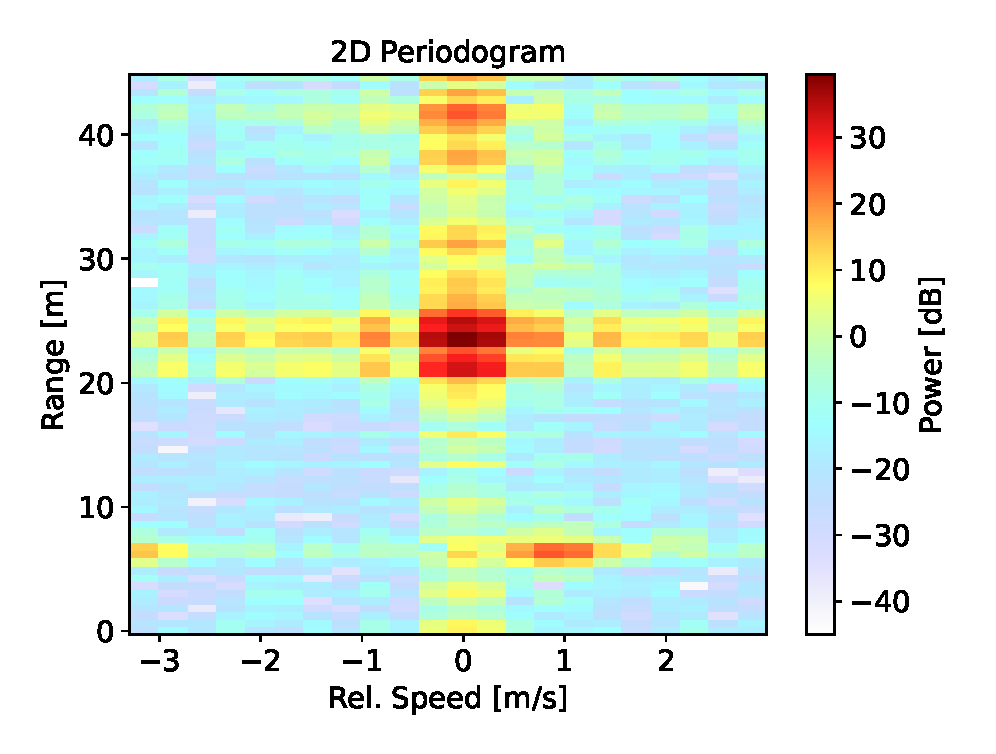
\includegraphics[scale=0.45]{Images/radar_detect_threshold/cfar_abv_thresh_PER.eps}%
				}
				
				\caption[]{Example of CFAR thresholding, it can be observed that the largest target positioned at 23 m (a wall) presents strong sidelobes that are detected as target returns.}
				\label{fig:RadThesh_CFAR_abv_thresh_doubl}
			\end{figure}
			
			
			One common method for significantly reducing false alarms after the detection process is using a confirmation system that requires each target to be detected twice: once in the initial search and in a subsequent confirmation process.
			However, there is still the possibility that a noise spike will remain in the confirmation measure and the target will not. In addition, this approach can suffer from peaks generated by clutter or spectral artefacts that may persist over time.

		\subsection{Cell-averaging CFAR}
		\label{sec:cell averaging CFAR}

The generic CFAR detector described in the previous section defines a threshold, based on noise power, to be applied to the whole periodogram. More advanced algorithms for CFAR detection belong to the family of cell-averaging CFAR (CA-CFAR) \cite{Richards_2014}.

In a noisy environment, very weak echo signals may be lost in the case of a fixed threshold across the periodogram. CA-CFAR estimates the threshold level for each cell of the 2D periodogram based on the statistics of neighbouring cells belonging inside a set reference window. In this way noise levels are estimated for smaller sections of the periodogram, adapting to the local level of the interference and defining a variable threshold across the periodogram.

The CFAR window resides inside the data window and is composed of leading and lagging reference windows, guard cells and cell-under-test (CUT). Guard cells are discarded for noise computation since they may contain returns associated with the target in the CUT.

In the OFDM range-doppler radar problem a two-dimensional CFAR window is considered, where the CUT is located at the center.

\begin{figure}[H]
	\centering
	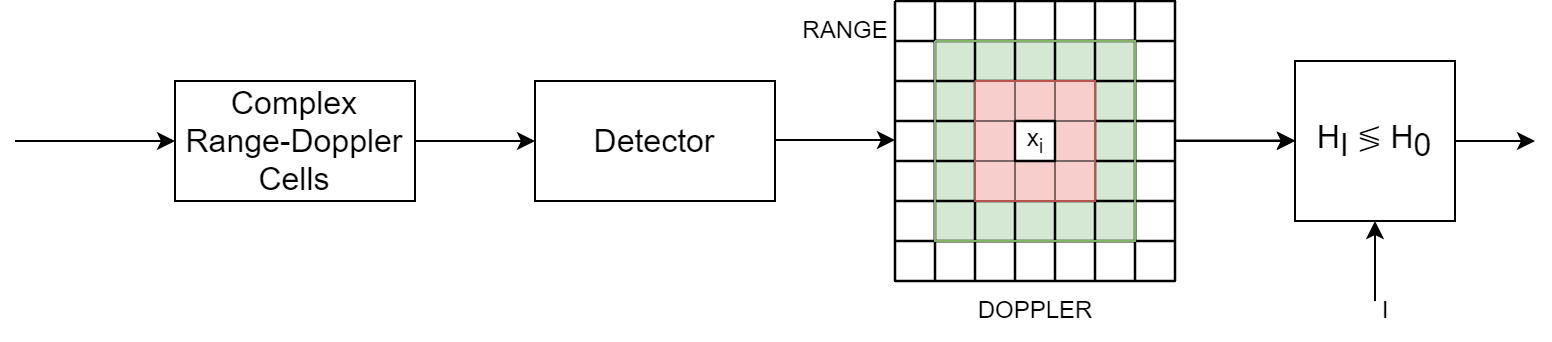
\includegraphics[width=0.9\textwidth]{Images/radar_detect_threshold/cacfar_pipeline.png}
	\caption{CA-CFAR detection processor, guard cells are indicated in red, while reference cells are highlighted in green.}
	\label{fig:cacfar_pipeline}
\end{figure}


% TODO: insert CACFAR scheme from presentation (add guard cells)
% TODO: insert sliding windows

The CA-CFAR threshold is defined by the product of the noise power estimate and a CFAR constant

\begin{align*}
	T = \alpha_{\text{CA}} \hat{\sigma_N}^2.
\end{align*}

The CFAR constant $\alpha_{\text{CA}}$ is a function of the probability of false alarm $p_{\text{FA}}$ and of the number of contribution cells $N$ and is derived as in chapter 16.5 of \cite{Richards_Scheer_Holm_2010}. The estimated noise power is calculated as in \ref{align: threshold_noise_power} by averaging over the contributing cells

\begin{align*}
	\alpha_{\text{CA}} =& N[p_{\text{FA}}^{-1/N} - 1] \\
	\hat{\sigma_N}^2 =& \frac{1}{N}\sum_{n=1}^N z_n.
\end{align*}

The number of operations can be reduced by simplifying the normalization by $\frac{1}{N}$ by defining a noise statistics $\hat{g}_{\text{CA}}' = \sum_{n=1}^N z_n$ and by incorporating it in the CFAR constant $\alpha_{\text{CA}}' = p_{\text{FA}}^{-1/N} - 1$.

Computationally CA-CFAR is more demanding than other thresholding techniques, as in its fastest implementation it still requires a 2D convolution to be applied to the periodogram before computing the threshold at each bin.

\subsubsection{Performance of CA-CFAR}

The general assumption that each radar return occupies one single bin in the range-Doppler plane is not valid for OFDM radar systems, as the \gls{psf} is influenced by a number of factors.
Zero padding and windowing in the periodogram define the width of the main lobe of the sinusoids in the 2D plane, while a large time aperture of the acquisition generally leads to a larger return due to range and Doppler spreading.
Furthermore, spread targets generate bigger responses than a point scatterer, impacting neighbouring periodogram bins.

In a heterogeneous radar frame multiple targets and changes in the interference power degrade CFAR performance. If target returns are present in the reference window, they will bias the threshold and lead to a missed detection. This phenomenon is called \textit{target masking}. Another source of performance degradation is the presence of clutter, where \textit{clutter boundaries} are zones inspread targets generate
bigger responses than a point scatterer, impacting
neighbouring periodogram bins which there is a sudden change in the statistics of the interfering power, which leads to higher threshold and missed detection.

Performance is also strongly influenced by the design of the reference window. The window should be designed to be as small as possible, in order to reduce the computational load due to the convolution operation and not to include interfering statistics far away from the CUT. The guard interval should be dimensioned according to the point spread function of the target return. An extended target could be counted in the reference window and lead to \textit{self masking}.

	\begin{figure}[H]
		\centering
		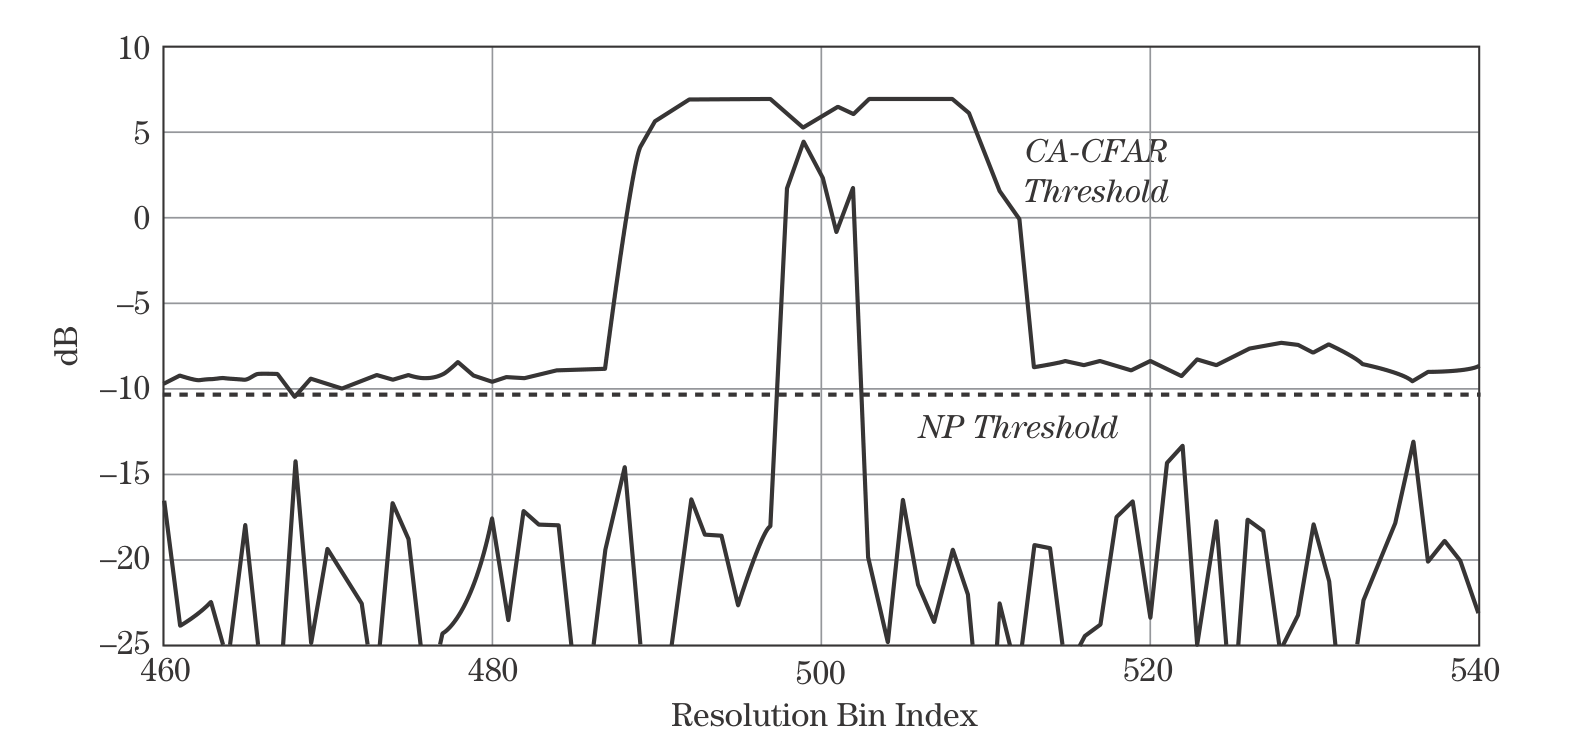
\includegraphics[width=0.7\textwidth]{Images/radar_detect_threshold/self_masking_Richards2010.png}
		\caption{Example of self masking in a 1D radar signal \cite{Richards_Scheer_Holm_2010}}
		\label{fig:self_masking_Richards2010}
	\end{figure}

	\begin{figure}[H]
		\centering
		
		\subfloat[Above-threshold bins using CA-CFAR.\label{fig:RadThesh_CA_CFAR_missed_detect}]{%
			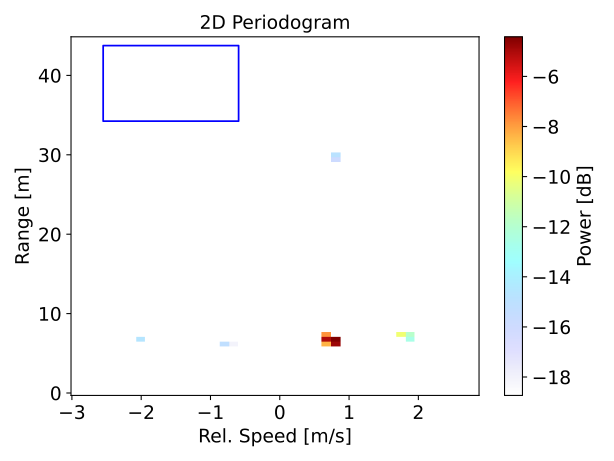
\includegraphics[scale=0.45]{Images/radar_detect_threshold/ca_cfar_no_nlos_1.png}%
		}\hfill
		\subfloat[Reference periodogram. LOS target at 6 m and corresponding NLOS path return at 40 m, -1,5 m/s.\label{fig:RadThesh_CA_CFAR_missed_detect_PER}]{%
			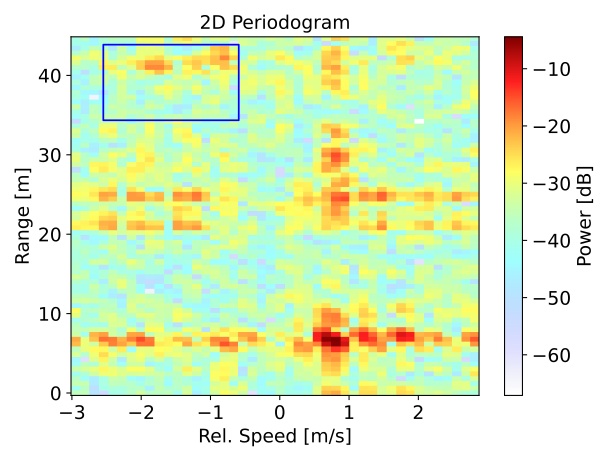
\includegraphics[scale=0.45]{Images/radar_detect_threshold/ca_cfar_no_nlos_PER_1.png}%
		}
		
		\caption[]{\small Clutter-like return observed in NLOS (top-left area denoted by the blue box): CA-CFAR uses part of the point cloud to estimate noise levels and the target is not detected.}
		\label{fig:RadThesh_CA_CFAR_missed_detect_doubl}
	\end{figure}

	In a NLOS sensing scenario, CA-CFAR suffers from these drawbacks due to the lower \gls{snr} of target returns caused by multiple reflections and the presence of strong static clutter components.
	Additionally, target returns can occupy multiple bins in the periodogram, leading to self masking. 
	As a result, they do not appear as distinct peaks, but rather are spread across neighbouring bins, which raises the CA-CFAR threshold and leads to missed detections, as shown in Figure \ref{fig:RadThesh_CA_CFAR_missed_detect_doubl}.

\subsubsection{Robust CA-CFAR}
More complex CA-CFAR algorithms may provide better results under certain heterogeneous conditions, but at the expense of increased computational complexity, higher cost, or lower performance under non-ideal conditions.

Some of the more common variations of the algorithm are the greatest-of CA-CFAR (GOCA-CFAR) and the censored statistics CA-CFAR (CSCA-CFAR), which are designed to suppress clutter-edge false alarms and mutual target masking, respectively.

\paragraph{Greatest-of CA-CFAR:}
the interference power is calculated in the lagging and leading reference windows separately and the largest of the two is selected as the reference statistics. In the OFDM radar signal the leading/lagging definition can be applied only in the doppler dimension, since interference statistics is assumed homogeneous in range.

GOCA-CFAR can, in general, avoid false alarm caused by clutter returns and clutter-edge conditions. However, in NLOS sensing, where the power of the target returns is comparable to the one of spectral artifacts and clutter sidelobes, GOCA-CFAR increases the possibility of masking, especially for slow-moving targets.
 
 
\paragraph{Censored-statistics CA-CFAR:}
this algorithm considers the largest $N_c$ samples to be containing returns from interfering targets, and therefore does not consider them when computing the interference statistics. CSCA-CFAR is in general assumed to be capable of removing up to $N_c$ interfering targets.
This algorithm can be also generalised by censoring an arbitary number of samples in order to be adapted to different environments. 

The main limitation posed by this algorithm is the increased computational cost due to the necessary ordering of the interference samples.


\subsection{Range-adjusted exponential threshold}

	
	In \cite{Wagner_Feger_Stelzer_2017}, a different approach to thresholding was proposed for detecting large point clouds of radar returns in the 2D range-Doppler plane. Similar to the OFDM radar case in this work, due to the relatively high speed resolution, returns occupy multiple cells in the periodogram and are not correctly detected by CA-CFAR.
	
	The idea is to adjust the threshold level accounting for the propagation loss of the target reflection, which is proportional to the square of the distance from the transmitter. 
	
	This solution was implemented combining the CFAR threshold, set as a lower bound, and the range-dependent exponential adjustement.
	
	The threshold for a range-bin corresponding to returns at range $d$ is
	
	\begin{align*}
		\eta_{\text{exp}} = \eta_{\text{CFAR}} + \frac{\alpha}{d^2},
	\end{align*} 
	
	where $\alpha$ is an adjustment factor for the exponential term. For this particular implementation it was defined as the square root of the maximum return in the periodogram
	
	\begin{align*}
		\alpha = \sqrt{\max{ \left\{\text{Per}_{\bm{F}}(n,m)\right\} }}.
	\end{align*}
	
	Unlike CA-CFAR where, in general, local peaks are dected, this approach will select large point clouds whithin the periodogram, as highlited in Figure \ref{fig:RadThesh_exp_thresh}.
	Targets can then be detected by searching for local peaks in the areas above threshold. A more refined result can be obtained by applying clustering algorithms, such as DBSCAN.
	
		\begin{figure}[H]
		\centering
		
		\subfloat[Periodogram with target at 9 m, moving at 1 m/s. Sidelobes from the target are present.\label{fig:RadThesh_exp_thresh_baseline}]{%
			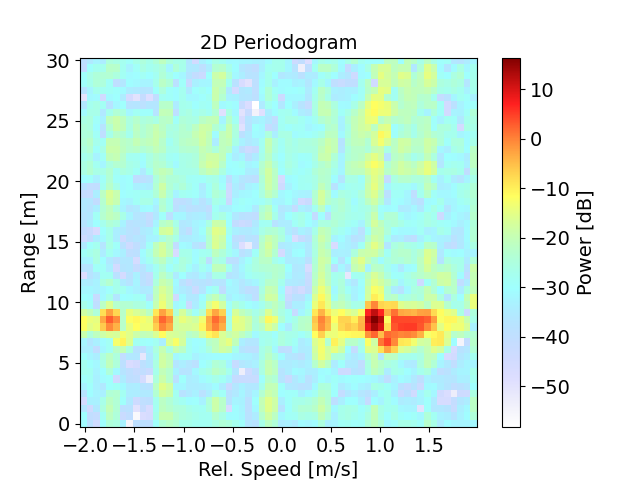
\includegraphics[scale=0.45]{Images/radar_detect_threshold/exp_thresh/per_NO_thresh.png}%
		}\hfill
		\subfloat[Above-threshold periodogram, after applying exponential threshold.\label{fig:RadThesh_exp_thresh_above}]{%
			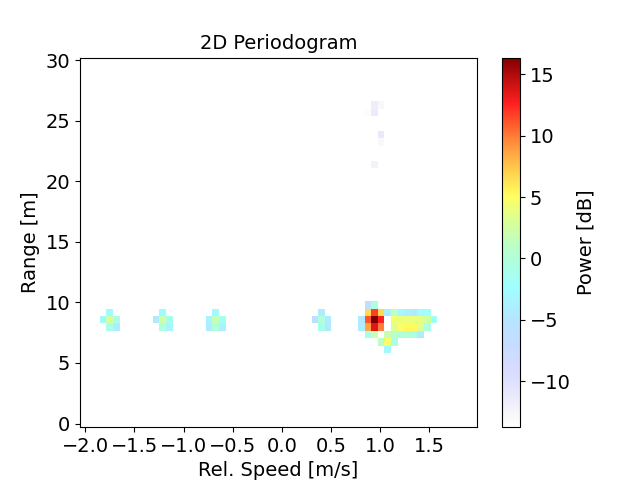
\includegraphics[scale=0.45]{Images/radar_detect_threshold/exp_thresh/per_exp_thresh.png}%
		}
		
		\caption[]{Example of detection using the proposed range-adjusted threshold.}
		\label{fig:RadThesh_exp_thresh}
	\end{figure}
	

\section{Clutter removal}
\label{sec:clutter_removal}

	Clutter removal in radar systems refers to the process of mitigating or eliminating unwanted signals or interference that arise from various sources (such as terrain, sea, or atmospheric conditions) and can obscure the detection of true radar targets.
	In general it is possible to refer clutter as any unwanted reflection from targets that are not of interest for the radar scope \cite{Richards_Scheer_Holm_2010}.
	
	In this work two existing implementations of clutter removal algorithms were applied to the CSI matrix.
	Both of them work by projecting the signal into a subspace orthogonal to the clutter.
	
	Both algoritms make use of an offline clutter acquisition step, performed before the sensing task. This step is used to gather information about clutter to be removed at runtime.
	
	\paragraph{Extensive Cancellation Algorithm by Subcarrier (ECA-C):}
	This algorithm, described in \cite{Wan_Cheng_Gong_Zhao_Shao_2012}, applies ECA \cite{Colone_ECA_2009} on each subcarrier of the CSI matrix.
	This approach is successful in removing the static clutter from the periodogram, at the cost of losing information on static targets and applying some distortion to targets moving at low speed.
	
	
	\paragraph{Clutter Removal with Acquisitions Under Phase Noise (CRAP):}
	CRAP introduces a novel approach by vectorizing the \gls{csi} matrices and preserving all information in both domains, unlike ECA-C which only works on each subcarrier separately and focuses solely on the time domain of the signal \cite{Henninger_CRAP_2023}.
	
	A detailed comparison between the two approaches can be seen in Figure \ref{fig:Rad_clutter_crap-ecac}. CRAP is able to remove static clutter without distorting the position of the target.

	\begin{figure}[H]
		\centering
		
		\subfloat[\footnotesize no clutter removal, static metal target at range of ca. 10 m. Clutter at ca. 23 m.\label{fig:Rad_crap_ecac_base_static}]{%
			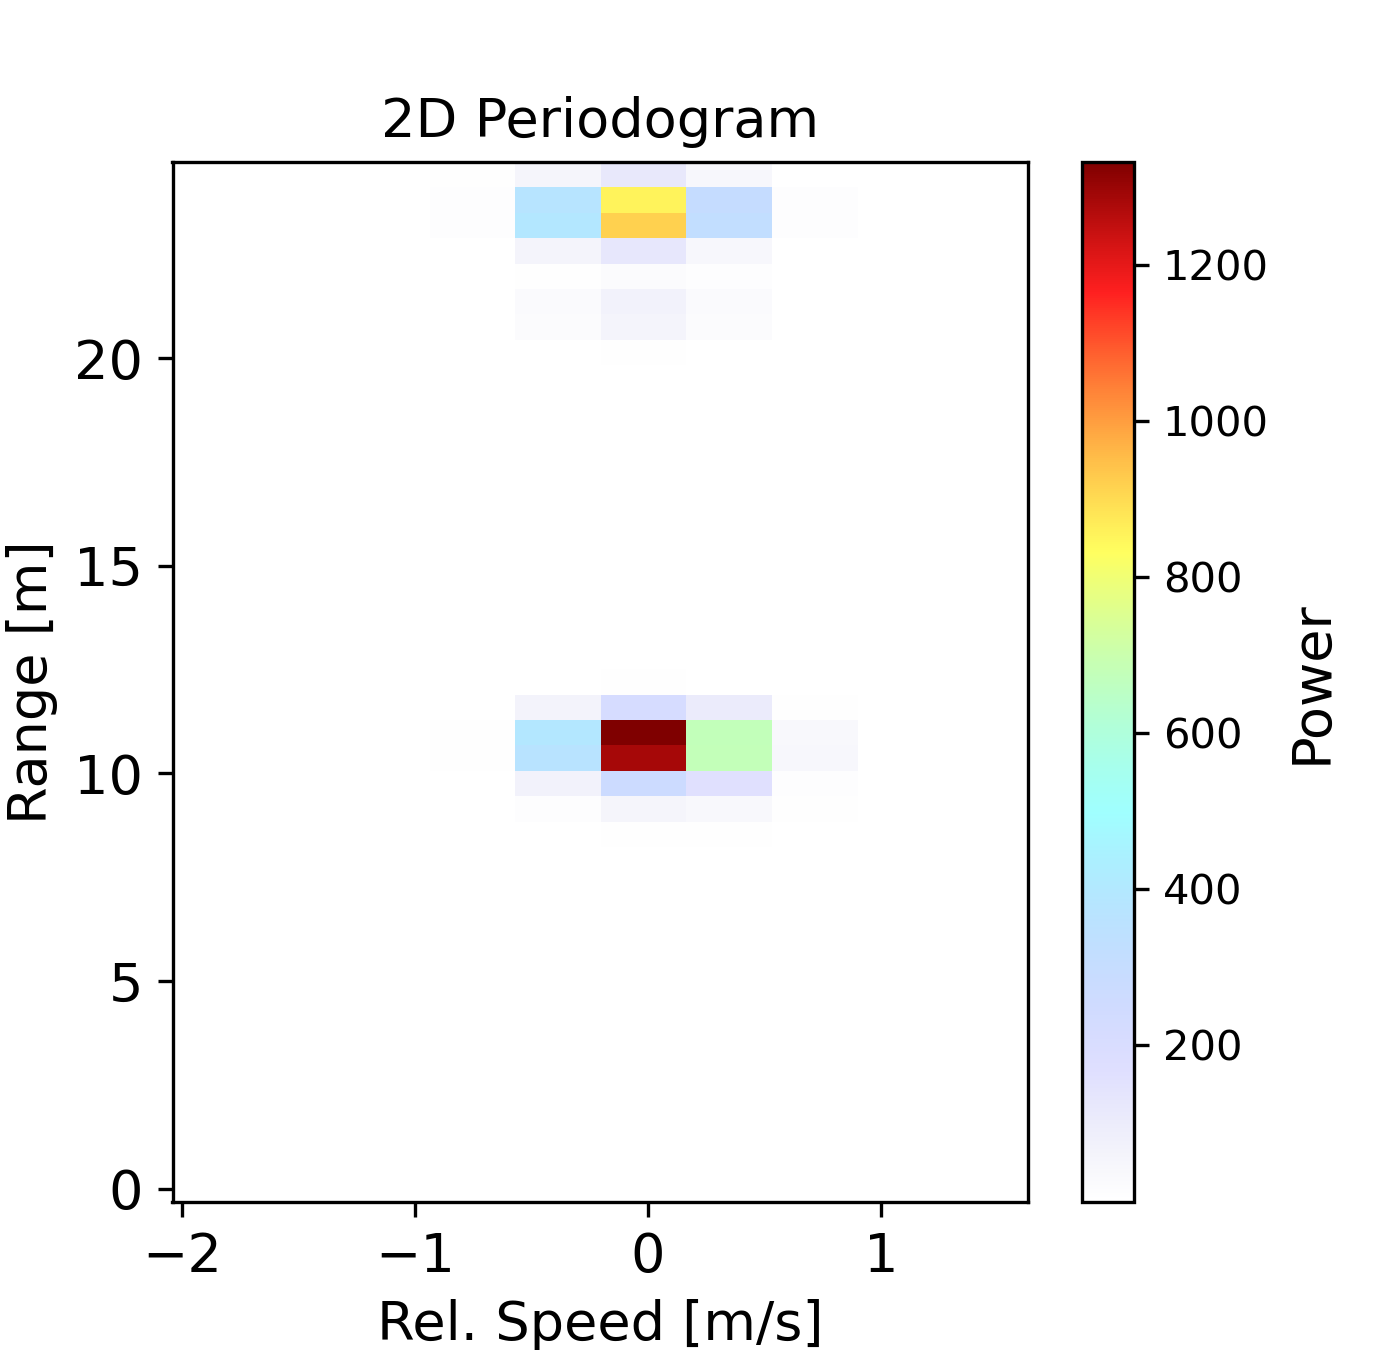
\includegraphics[scale=0.4]{Images/radar_detect_threshold/clutter/crap_ecac_static/clutter_baseline1.png}%
		}\hfill
		\subfloat[\footnotesize clutter removal with \newline ECA-C.\label{fig:Rad_crap_ecac_ECAC_static}]{%
			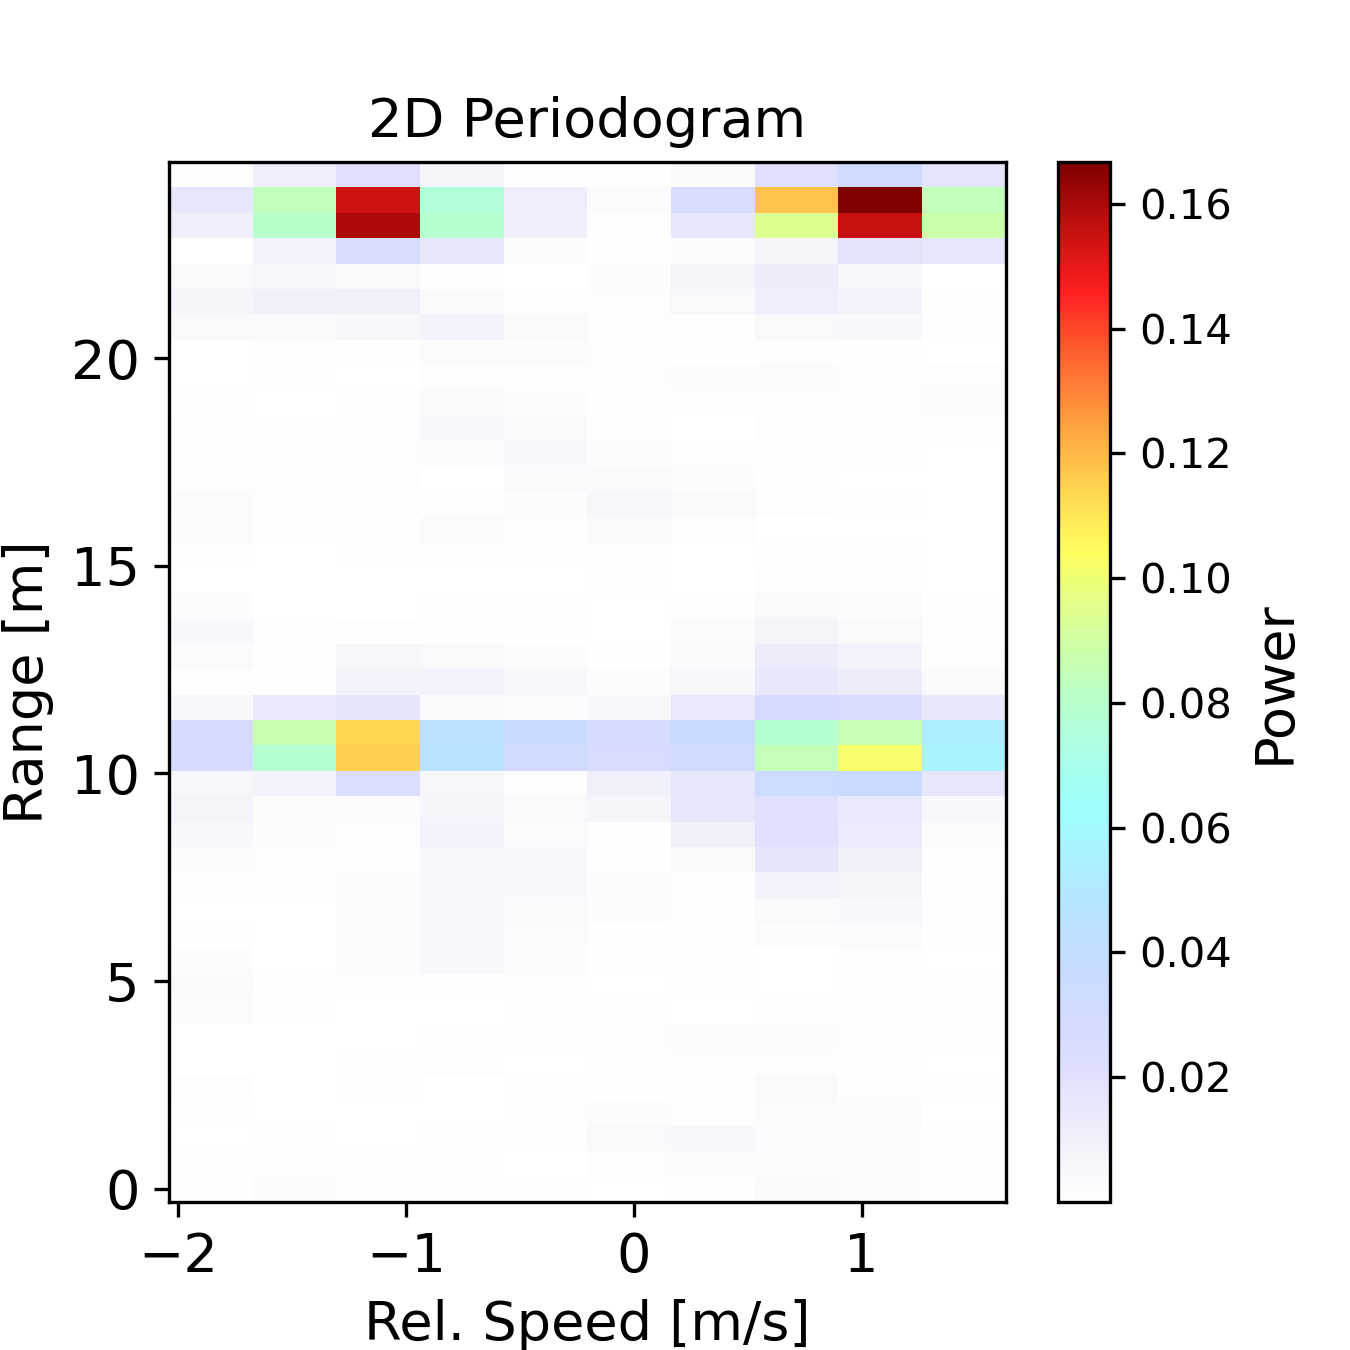
\includegraphics[scale=0.4]{Images/radar_detect_threshold/clutter/crap_ecac_static/clutter_ecac1.png}%
		}\hfill
		\subfloat[\footnotesize clutter removal using CRAP.\label{fig:Rad_crap_ecac_CRAP_static}]{
			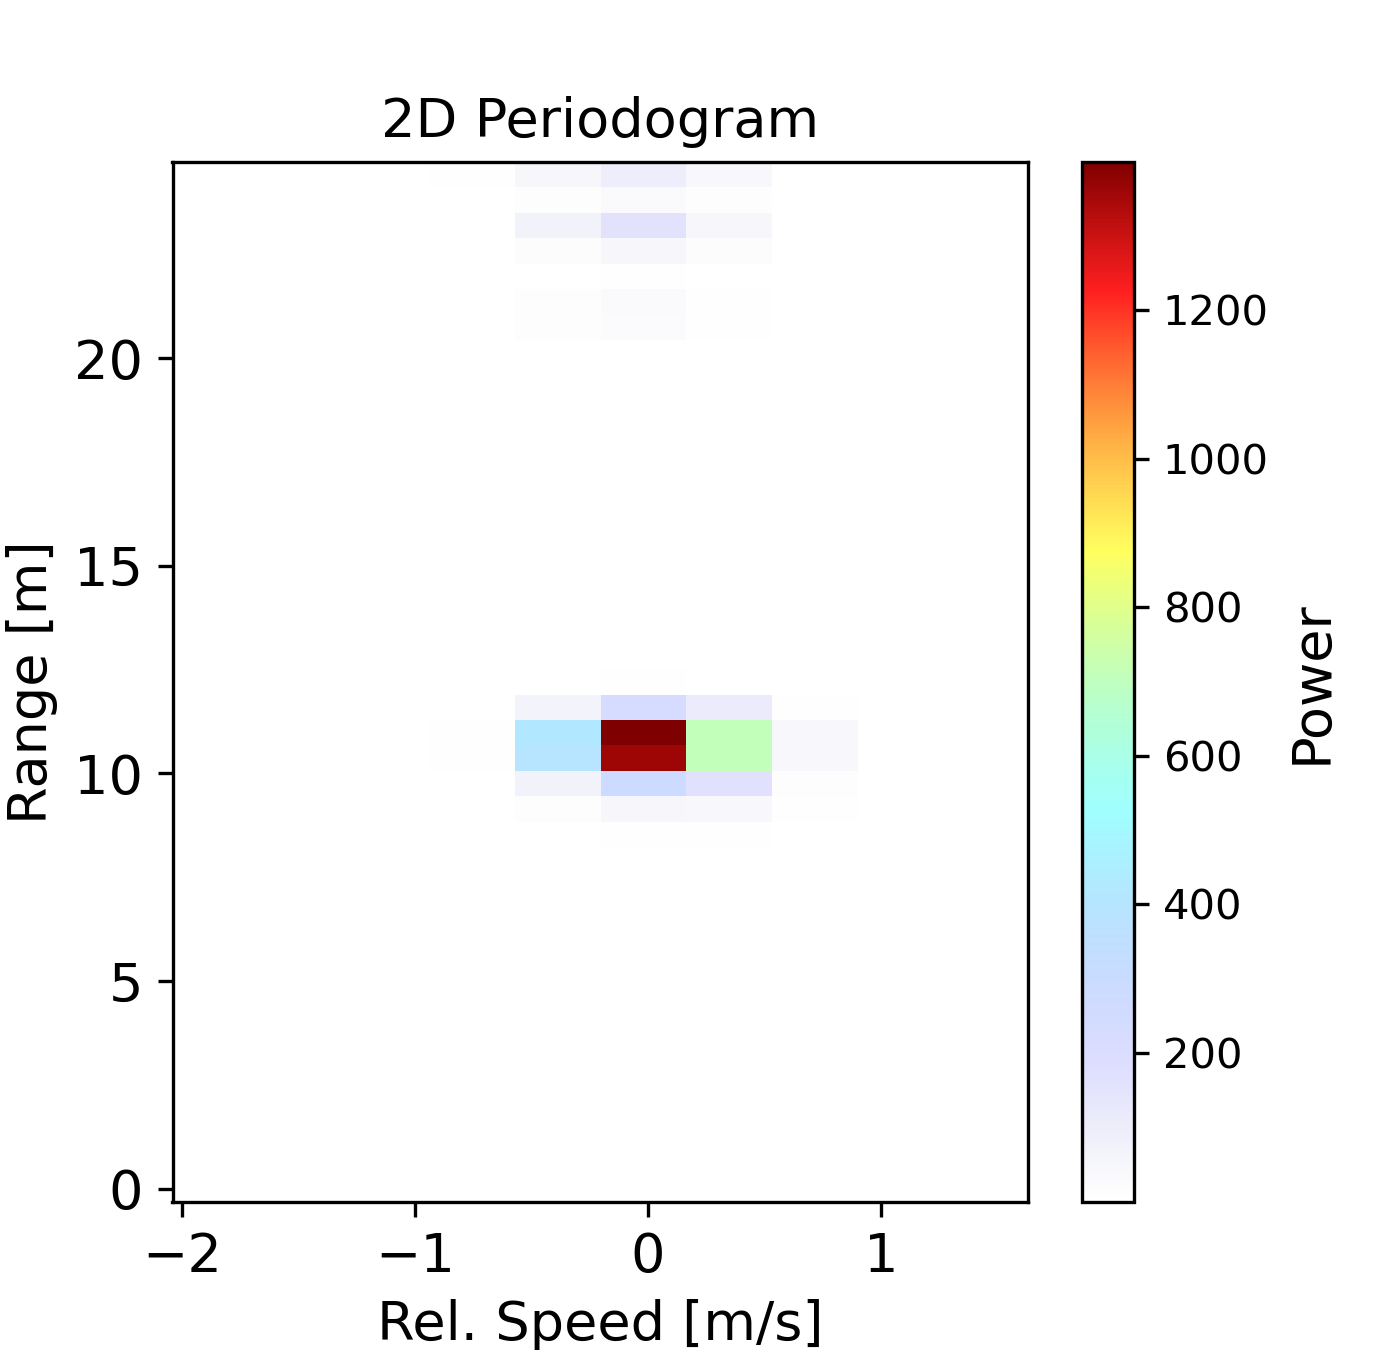
\includegraphics[scale=0.4]{Images/radar_detect_threshold/clutter/crap_ecac_static/clutter_crap1.png}
		}\newline
		
		\subfloat[\footnotesize no clutter removal, metal target at range of ca. 10 m moving at ca. 1 m/s.\newline Static clutter at ca. 23 m.\label{fig:Rad_crap_ecac_base_mov}]{%
			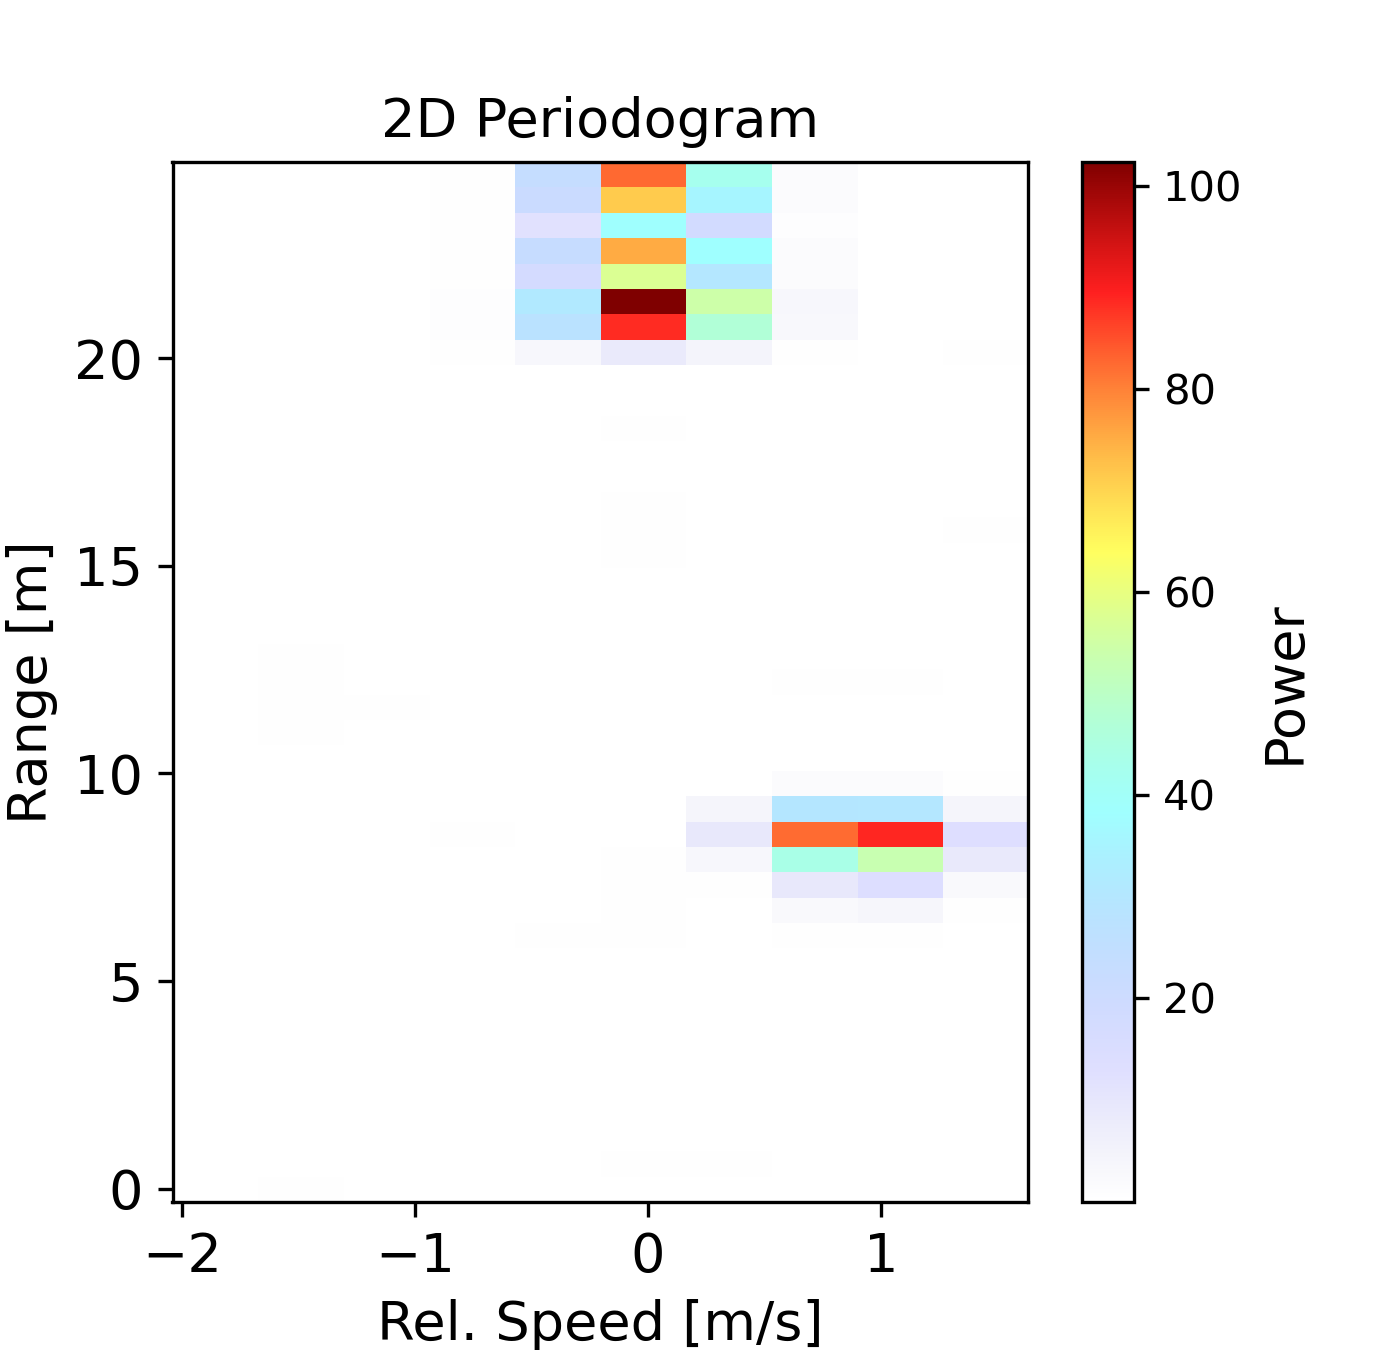
\includegraphics[scale=0.4]{Images/radar_detect_threshold/clutter/crap_ecac_mov/clutter_baseline_mov1.png}%
		}\hfill
		\subfloat[\footnotesize clutter removal with \newline ECA-C, moving target.\label{fig:Rad_crap_ecac_ECAC_mov}]{%
			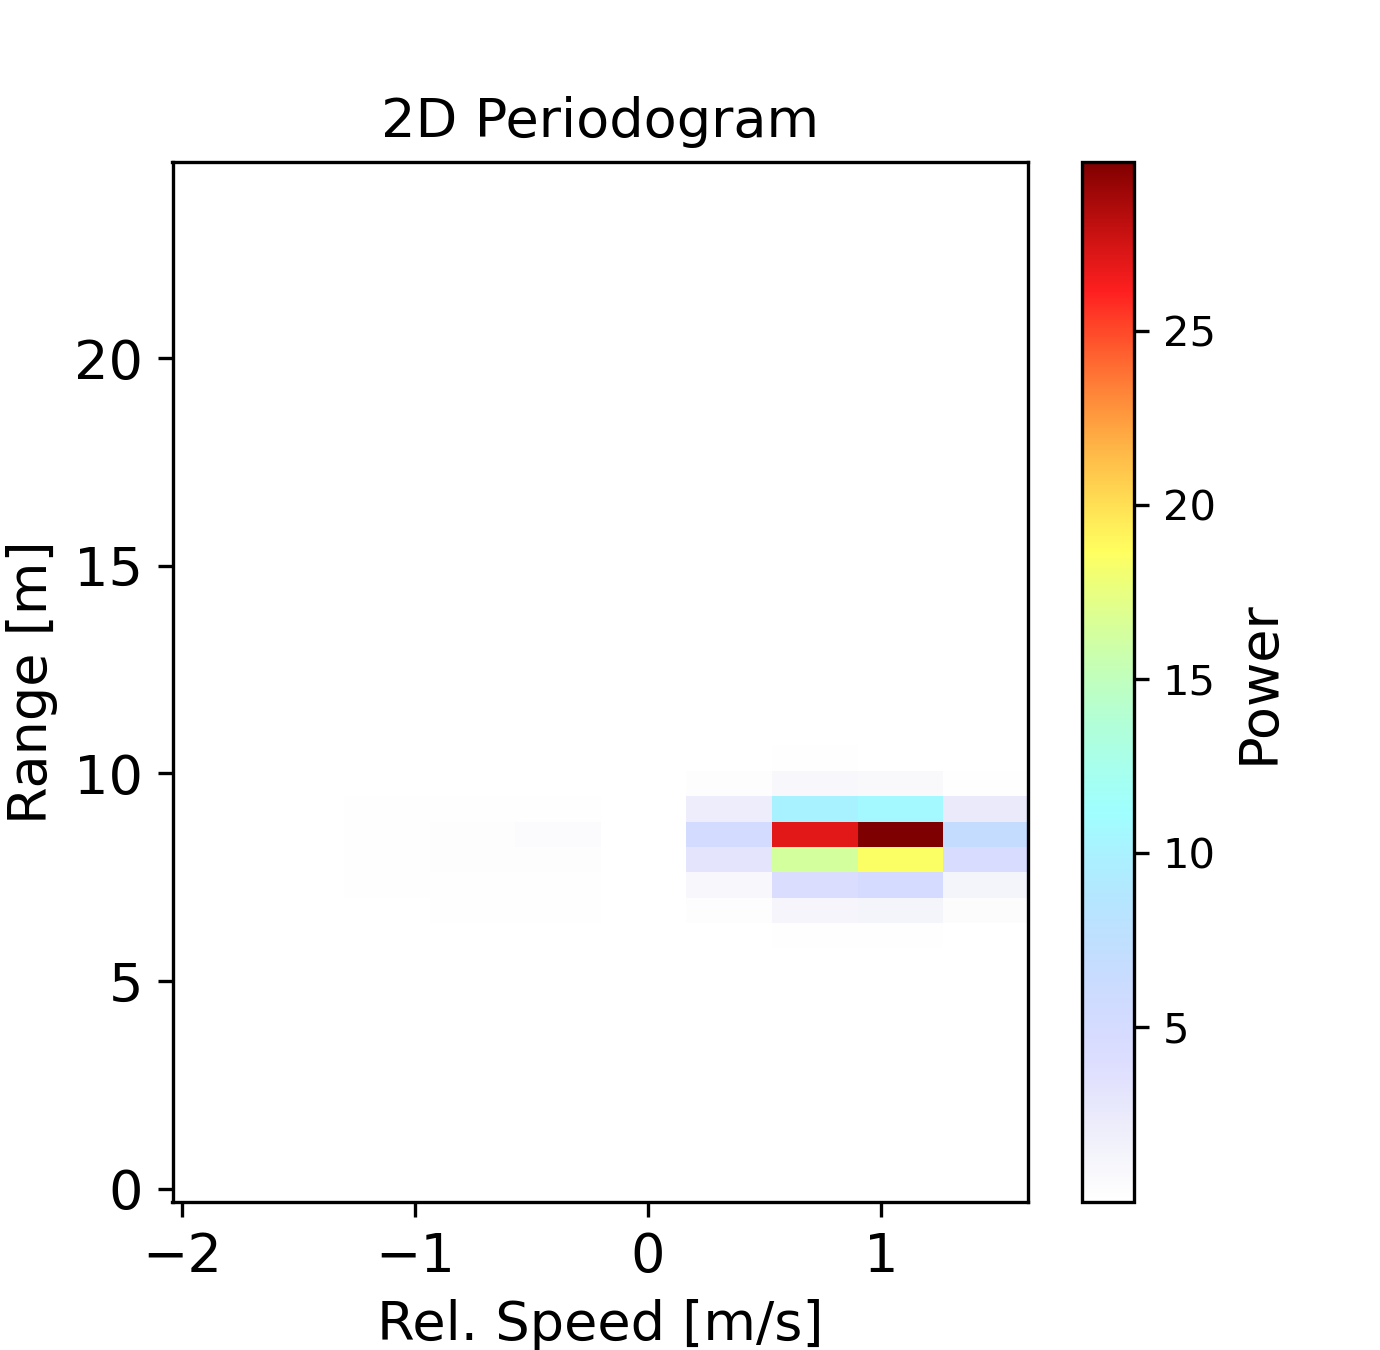
\includegraphics[scale=0.4]{Images/radar_detect_threshold/clutter/crap_ecac_mov/clutter_ecac_mov1.png}%
		}\hfill
		\subfloat[\footnotesize clutter removal using \newline CRAP, moving target. \label{fig:Rad_crap_ecac_CRAP_mov}]{%
			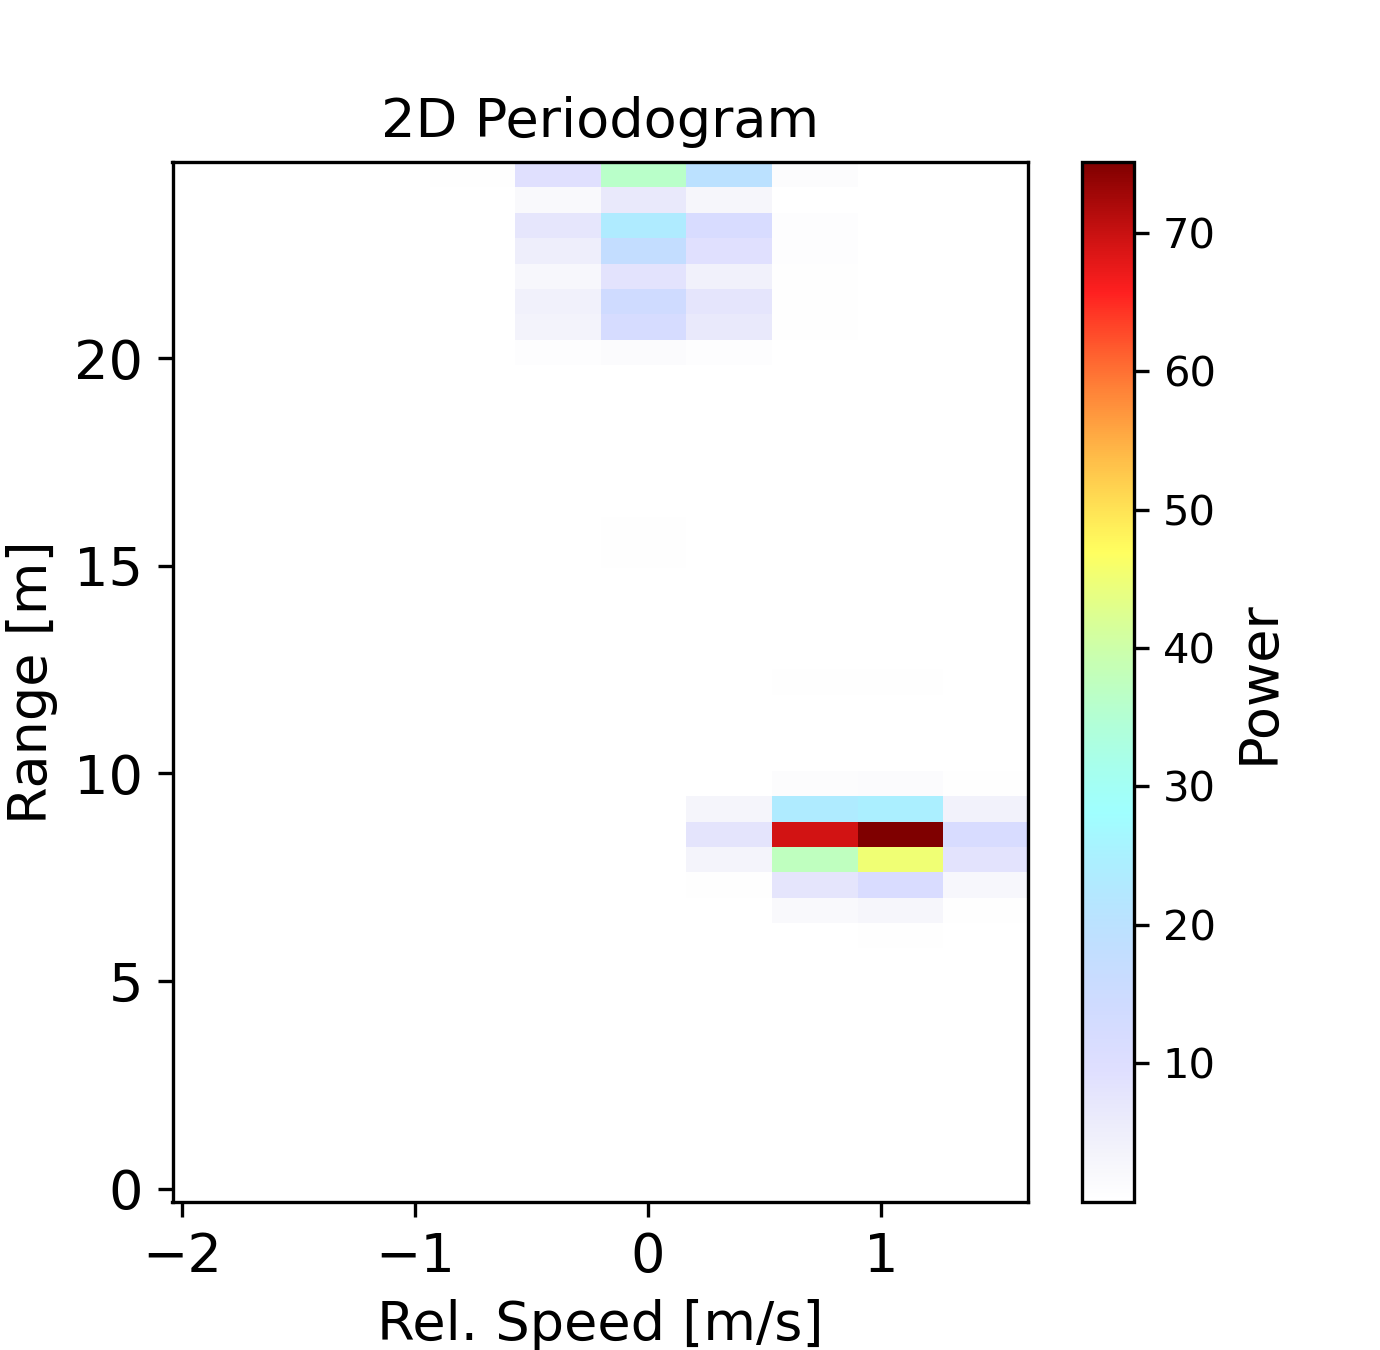
\includegraphics[scale=0.4]{Images/radar_detect_threshold/clutter/crap_ecac_mov/clutter_crap_mov1.png}%
		}
		\caption[]{\small Comparison of periodograms from sensing acquisitions obtained in NOKIA's indutrial test facility.
		Periodograms without clutter removal (left) are compared with those obtained after applying ECA-C (middle) and CRAP (right). It can be observed how ECA-C is able to clean the image from static clutter, albeit at the cost of losing information on static targets, as shown in \subref{fig:Rad_crap_ecac_ECAC_static}, whilst CRAP is able to retain the information.  }
		\label{fig:Rad_clutter_crap-ecac}
	\end{figure}
	
	\subsubsection{Clutter presence in NLOS}
	
	In a NLOS sensing setup, it is fairly easy to distinguish moving targets from the underlying noise floor.
	However, NLOS returns from static objects of interest will appear in the periodogram area where static clutter is more prevalent, as shown in Figure \ref{fig:Rad_clutter_comparison}.
	This makes the effective separation through radar thresholding and identification of the target difficult.

	\begin{figure}[H]
		\centering
		
		\subfloat[\label{fig:Rad_clutter_mov_target}]{%
			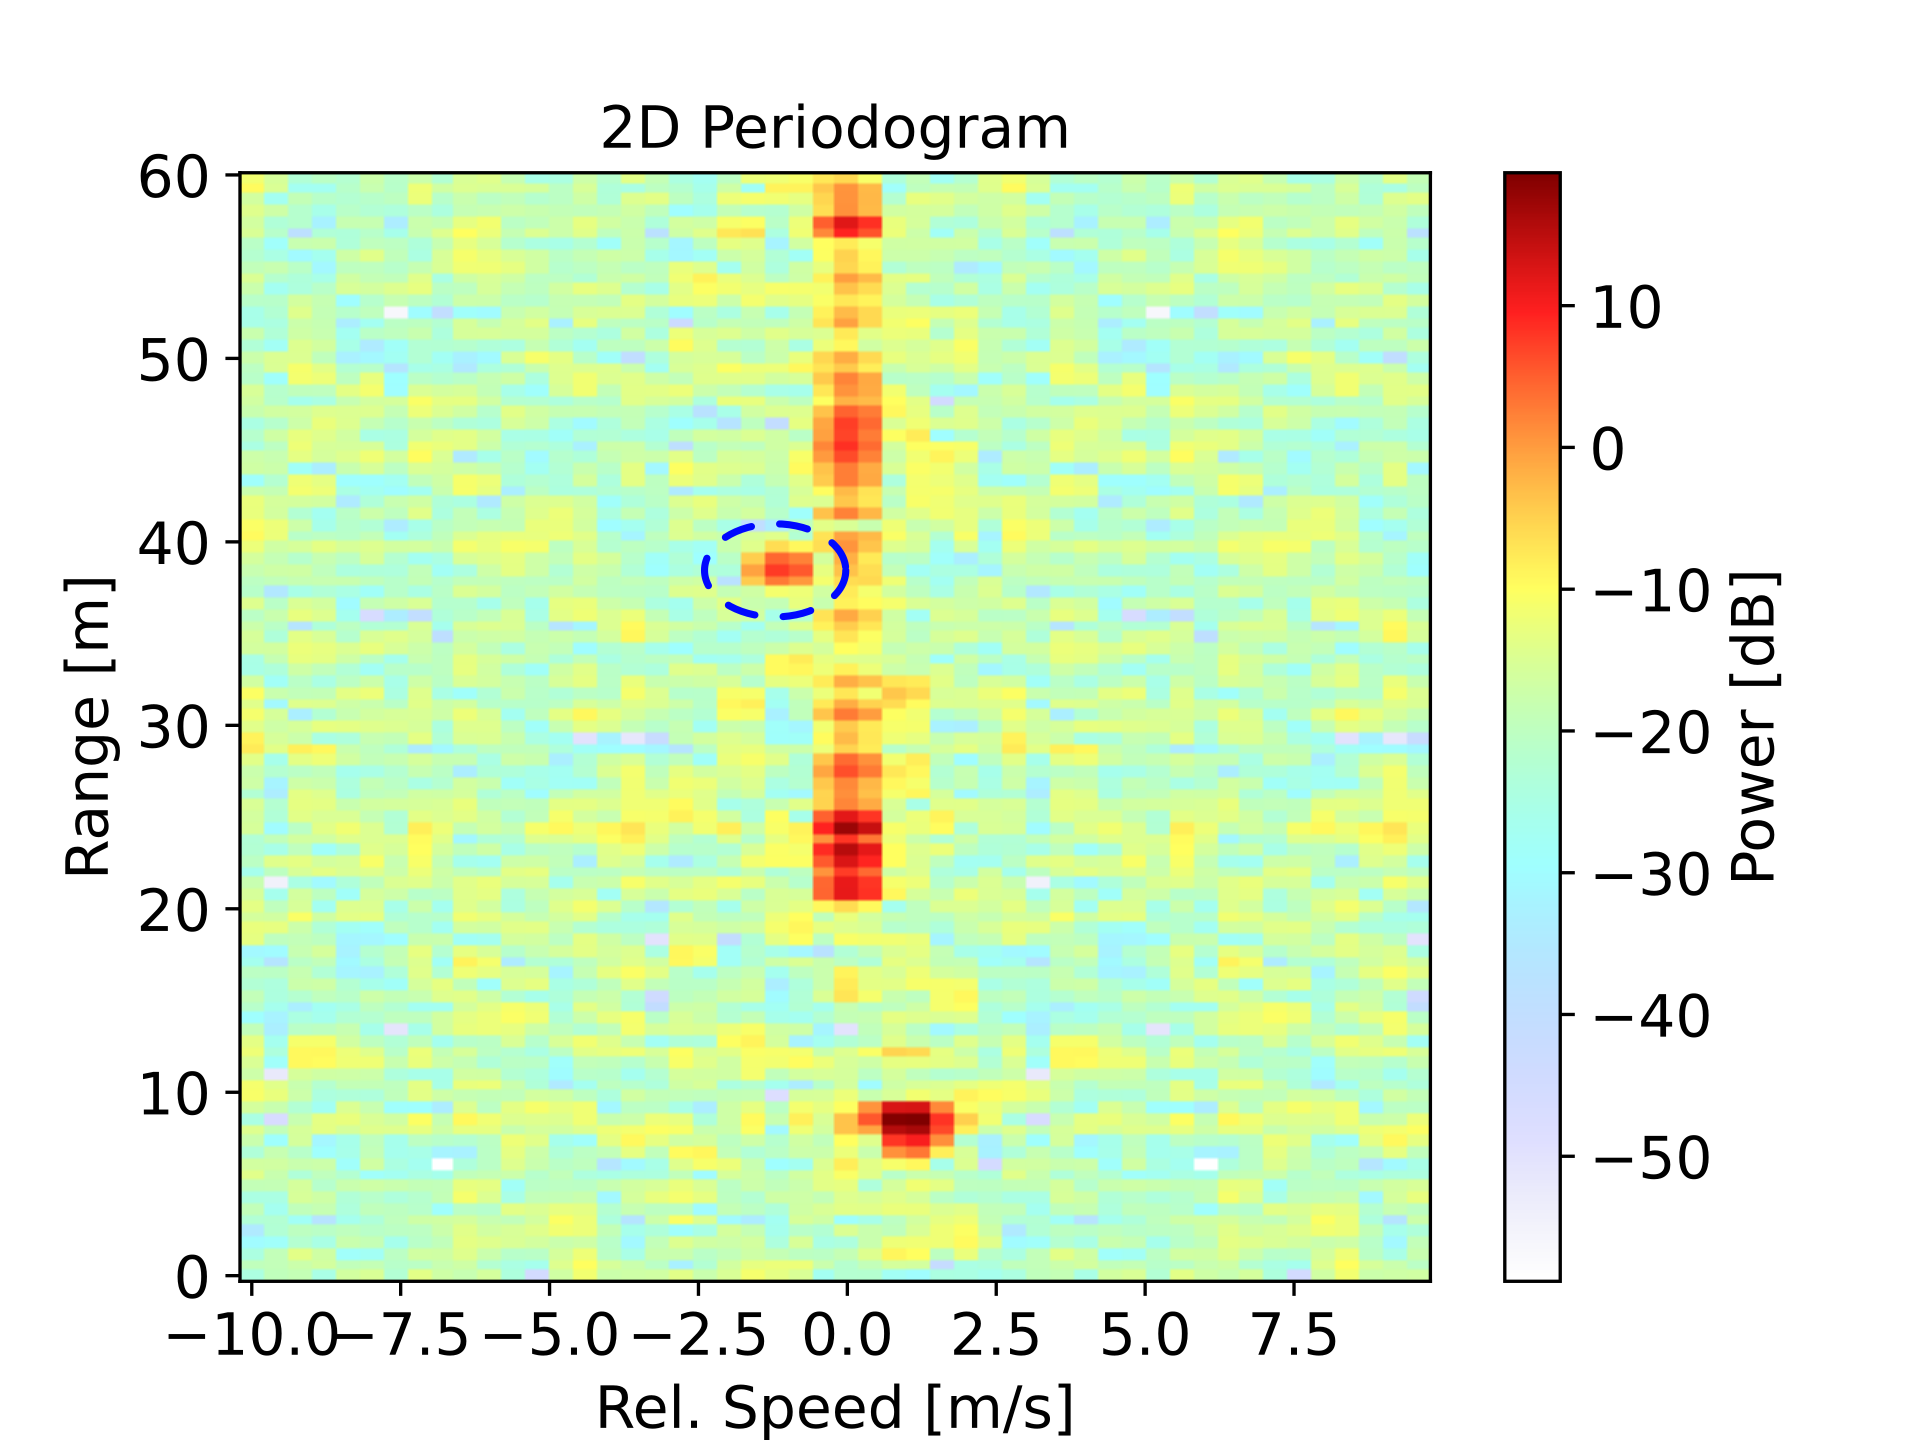
\includegraphics[scale=0.49]{Images/radar_detect_threshold/clutter/clutter_mov_target1.png}%
		}\hfill
		\subfloat[\label{fig:Rad_clutter_stat_target}]{%
			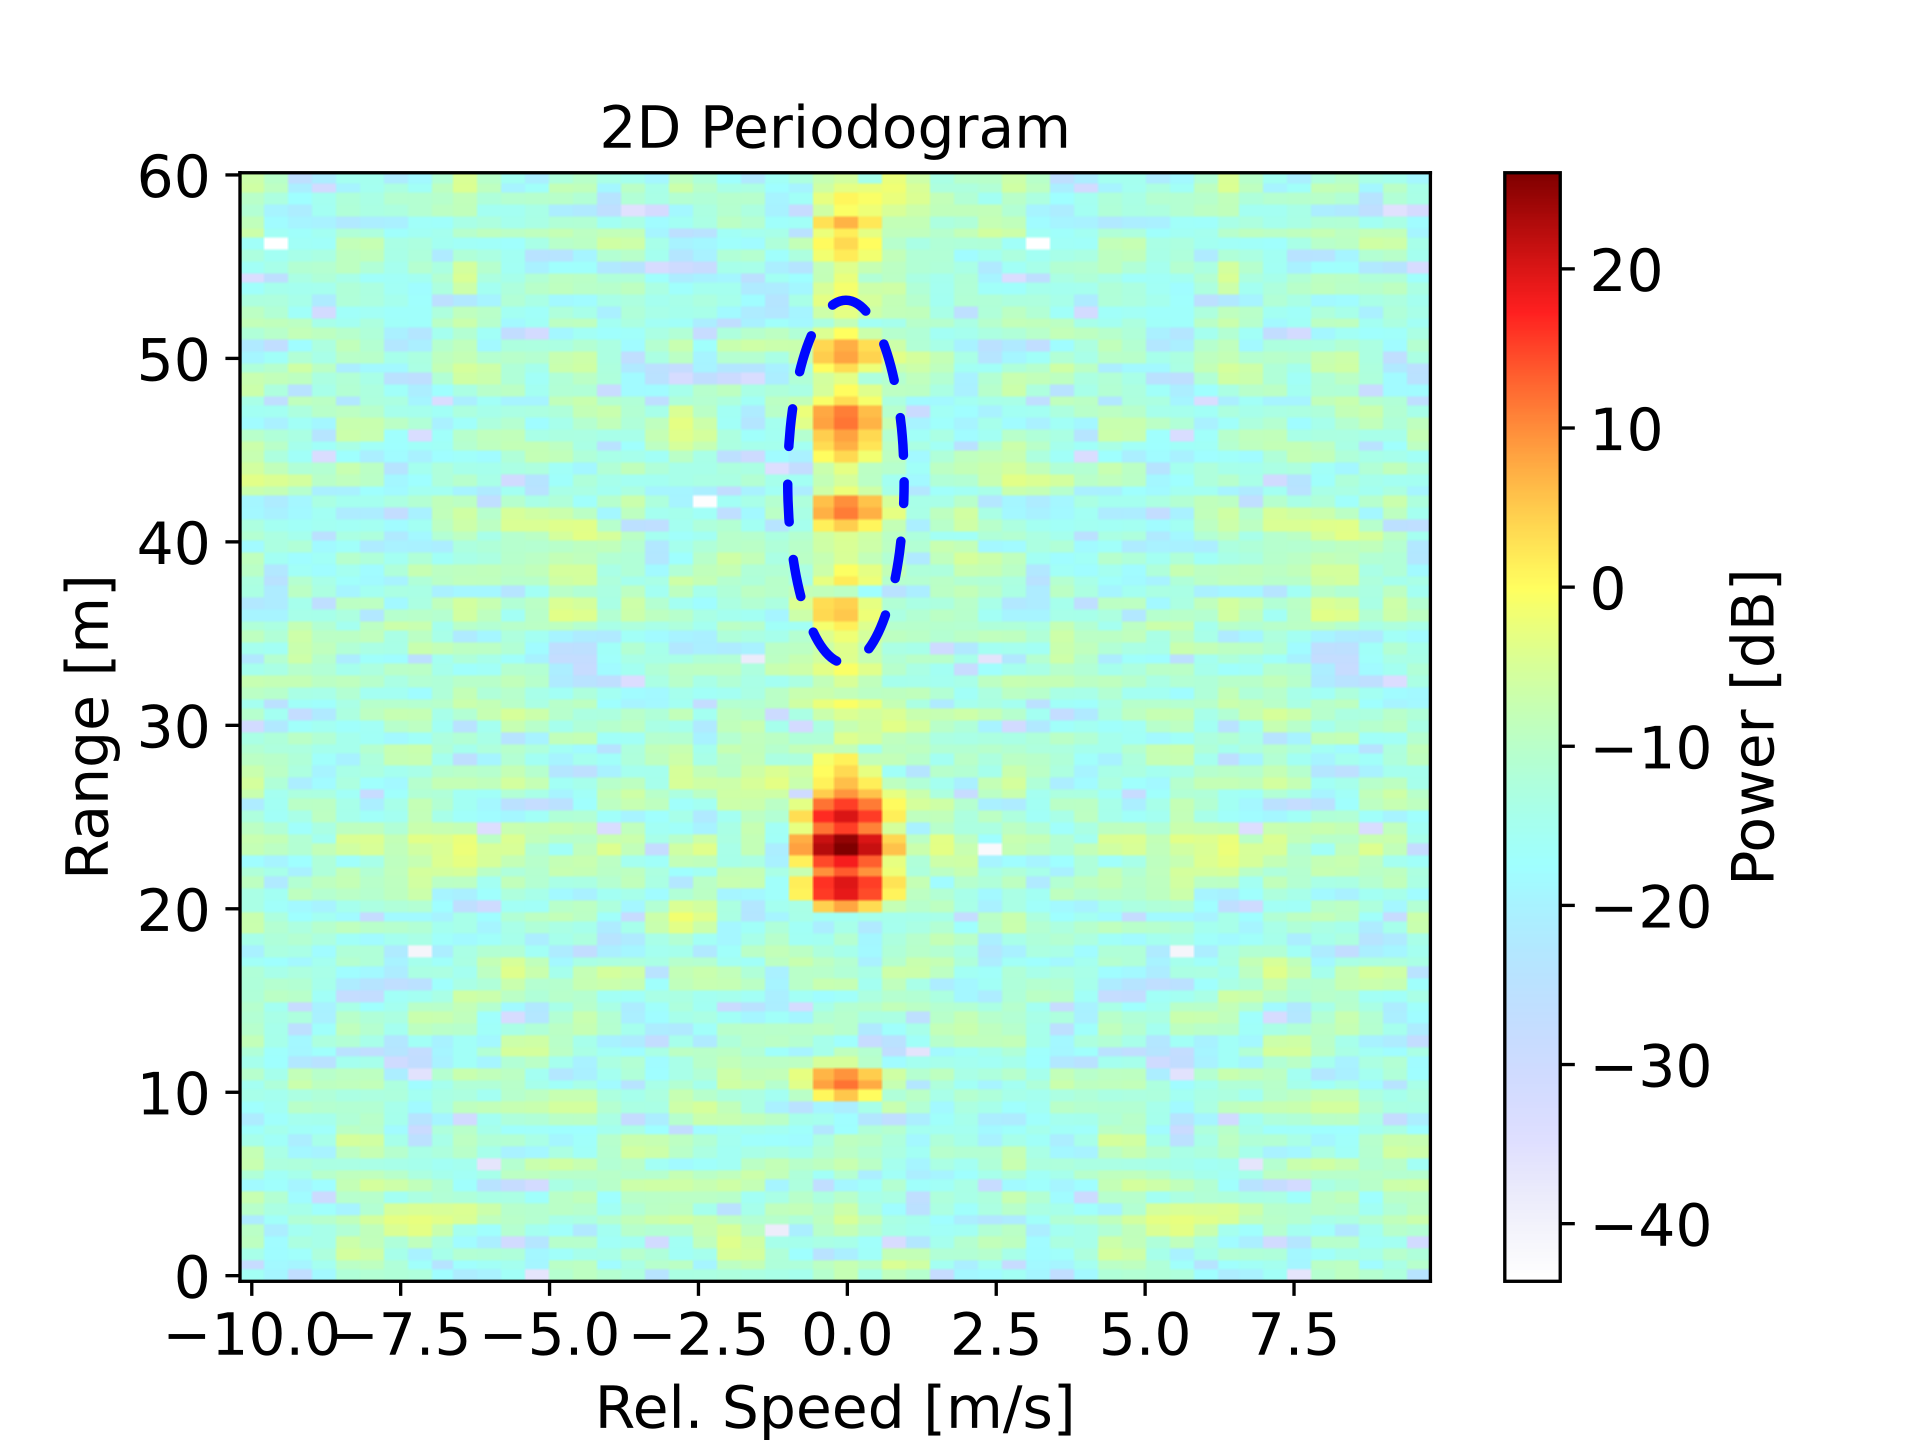
\includegraphics[scale=0.49]{Images/radar_detect_threshold/clutter/clutter_stat_target1.png}%
		}
		
		\caption[]{Periodograms with moving \subref{fig:Rad_clutter_mov_target}, and static \subref{fig:Rad_clutter_stat_target} targets in NLOS.
				Target is highlighted clearly when moving, while it appears as static clutter when it stops moving.}
		\label{fig:Rad_clutter_comparison}
	\end{figure}

	For intrusion detection purposes, it is sufficient to focus the radar search on moving targets. 
	Therefore, the static bins of the periodogram are discarded for NLOS processing.
	
	
	\section{NLOS-focused processing}
	\label{sec:nlos_proc_pipeline}
	
		\subsection{Line-of-sight and Non-line-of-sight separation}
		\label{sec:los_nlos_separation}
		
		
		
			In addition to clutter removal, calibration measurements provide valuable information for determining the distance threshold at which targets can be assumed to be in NLOS. 
			A portion of the calibration frames can be processed as radar frames, with a focus on the analysis of the zero-Doppler component.
			
			Shown in Figure \ref{fig:Test1_cali_static_per}, a target with large \gls{rcs} is present approximately $25$ m from the system. It was assumed that any return associated with a range greater than $25$ m was generated by a signal reflected from the largest static target. The figure also indicates that static clutter has a larger amplitude for ranges greater than $25$ m compared to lower ranges. This is due to the part of the beam that is reflected from the wall towards the environment and the associated returns.
			
			The distance between the gNB and the reflector of the NLOS components was estimated during the calibration step by averaging over the available measures.
			
			
			\begin{figure}[H]
				\centering
				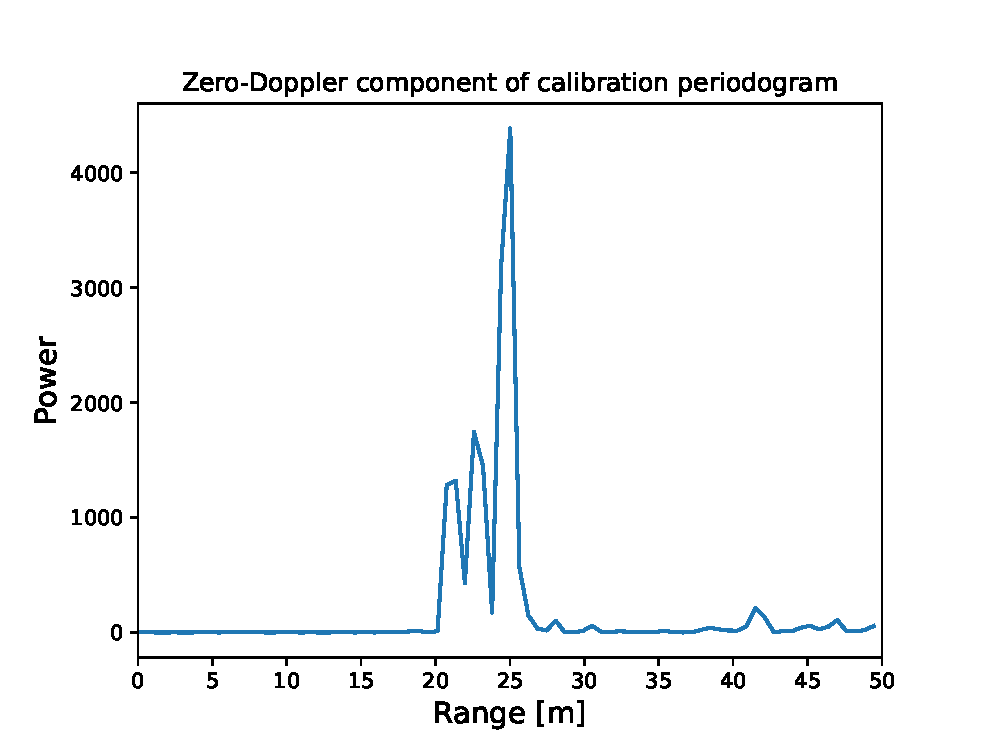
\includegraphics[width=0.6\textwidth]{Images/Test1/cali_static_per_t1.eps}
				\caption{\small Zero Doppler component of a periodogram generated from calibration measurements. It can be assumed that any returns detected beyond 25 m from the system are generated from multiple reflections and should be considered as NLOS components. }
				\label{fig:Test1_cali_static_per}
			\end{figure}
		
	
		\subsection{Modified periodogram}
		
			Figure \ref{fig:Rad_nlos_los_separation} highlights the regions of interest within the periodogram.
			The red area, which corresponds to static targets, is discarded. The periodogram is then divided horizontally into two regions, based on the range of the reflector for \gls{nlos}.
			
			\begin{figure}[H]
				\centering
				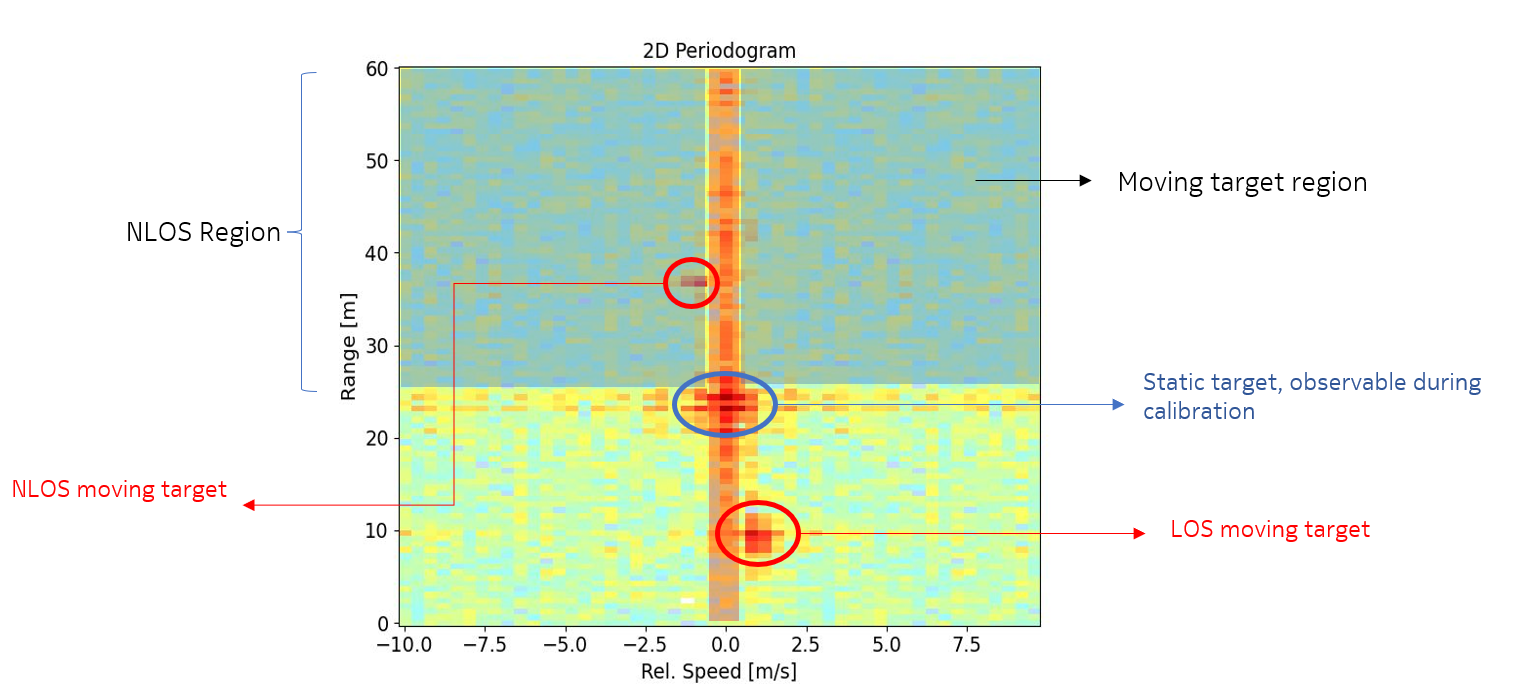
\includegraphics[width=1.1\textwidth]{Images/Test1/nlos-los-separation.png}
				\caption{\small Sample periodogram, separated in processing regions.}
				\label{fig:Rad_nlos_los_separation}
			\end{figure}
			
			
			After generating the periodogram, the processing phase can take into account this separation to process the \gls{nlos} section and \gls{los} section separately.
		
		\subsection{Processing of the NLOS region}
		
			After defining the two regions of interest from the periodogram and discarding the static components, as described in Section \ref{sec:los_nlos_separation}, peak detection and any additional processing can be conducted separately for each region. 
			
			Figure \ref{fig:Test1_NLOS-proc-pipeline} summarizes the proposed processing steps for NLOS sensing.
			
			%The chosen detection strategy was CA-CFAR, which utilized a square contribution window and a probability of false alarm $p_{\text{FA}} = 10^{-6}$. The size of the CA-CFAR window was set depending on the width of the target in speed bins, which depended on number of processed frames and OFDM sampled symbols.
			
			\begin{figure}[H]
				\centering
				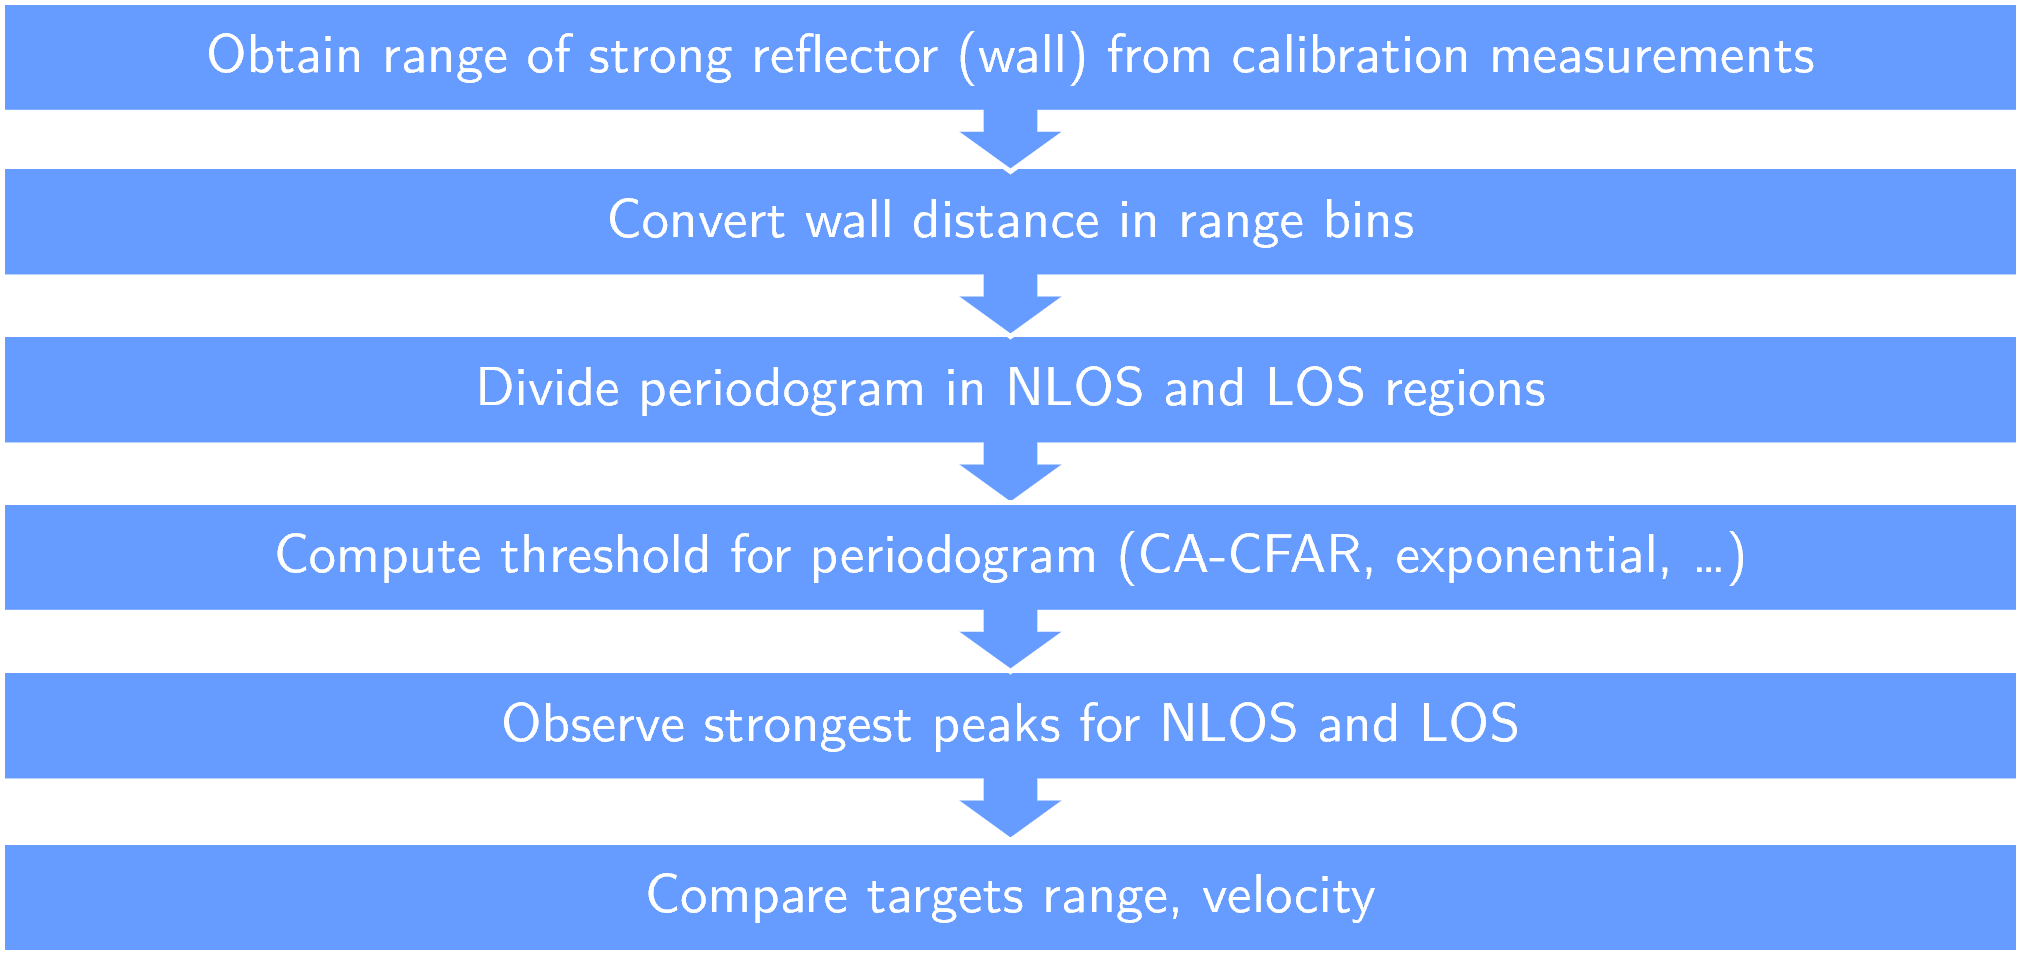
\includegraphics[width=0.8\textwidth]{Images/Test1/NLOS-proc-pipeline_wide_text12.png}
				\caption{\small Periodogram processing pipeline used for detection tests.}
				\label{fig:Test1_NLOS-proc-pipeline}
			\end{figure}
			
			
		 
			
			% TODO: add info on target dimensions for CA-CFAR, human case since guard cells were set in meters
			
		







